\subsubsection{Practical Informations}

Everything on the \href{https://moodle.epfl.ch/course/view.php?id=15697}{moodle}. A lot of exercises are taken from the Strogatz Book ("\textit{Nonlinear Dynamics and Chaos}" $2^\text{nd}$ edition). A solution book exists (M.Dichter, "\textit{Student Solutions for Nonlinear Dynamics and Chaos}"). The lectures from last year are available on \href{https://moodle.epfl.ch/course/view.php?id=15697#section-3}{SwitchTube}.

\subsection{The Lorenz Model}

\begin{figure}[h!]
    \centering
    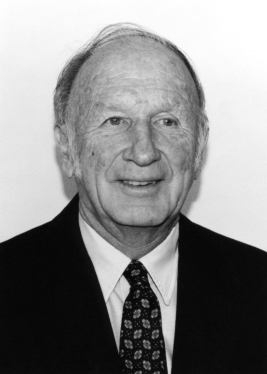
\includegraphics[width=0.4\textwidth]{figures/1_Edward_lorenz.jpg}
    \caption{Edward Lorenz.}
\end{figure}

We start "\textit{where everything started}": with the derivation of the Lorenz model. Edward Lorenz (1917-2008) was a mathematician who served as a meteorologist during the second world war. At the time, people linearized the fluid dynamics of the air. In his opinion, the system was intrinsically nonlinear. This lead to a key publication: [Lorenz, 1963] "\textit{Determinist Non-Periodic Flow}", which was first published in a meteorology journal, and is now the most-cited paper in chaos theory. It starts from a study of the convection in the atmosphere. \\

Let's see how he modeled convection cells. He looked at a 2D simplification of the problem.\\

\begin{figure}[h!]
    \centering
    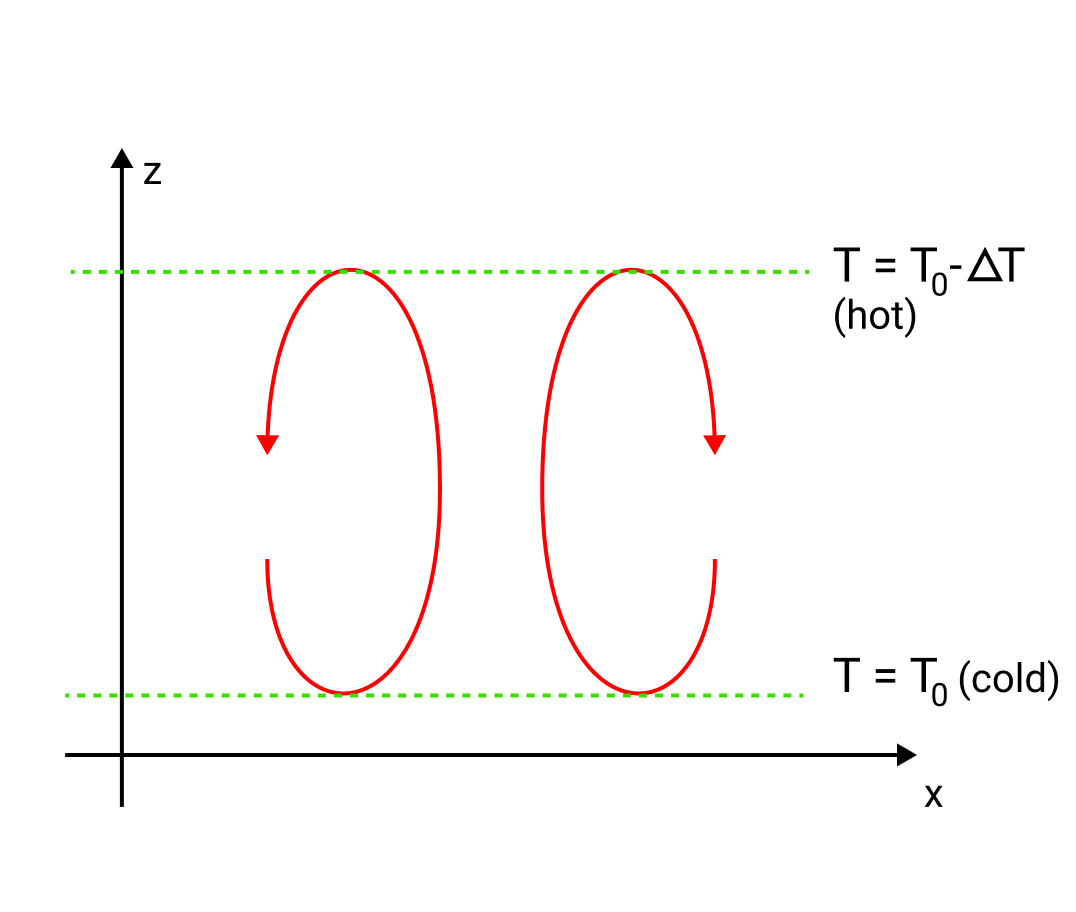
\includegraphics[width=0.7\textwidth]{figures/1_convection_cell.png}
    \caption{Convection cell model. Assume $\frac{\partial}{\partial y} = 0$ (i.e. a 2D approach).}
\end{figure}

We consider the velocity field $\vec{v} = u \vec{e}_x + v \vec{e}_y$. We start our derivation from:

\begin{enumerate}
    \item A continuity equation : $\frac{\partial \rho}{\partial t} + \nabla (\rho \vec{v}) = 0$. \\
    Since the flow is subsonic we can make the following (reasonable) approximation: $\rho = \text{constant}$. Which allows us to rewrite the equation as : 
    \begin{align}
        \nabla \vec{v} = \frac{\partial u}{ \partial x} + \frac{\partial w}{ \partial z} = 0  \tag{1}
    \end{align}
    \item A momentum equation (Navier-Stokes):\\
    \begin{align*}
        \overbrace{\rho \frac{D \vec{v}}{D t}}^\text{full derivative} 
        = \rho \left( 
            \frac{\partial \vec{v}}{\partial t} + \vec{v} \nabla \vec{v} \right) 
        = - \nabla \rho + \overbrace{\rho \vec{g}}^{= - \rho g \vec{e}_z} + \mu \nabla^2 \vec{v} 
    \end{align*}
\end{enumerate}

Let us introduce a new quantity: \textit{deviation from hydrostatic pressure}, which corresponds to $\rho = \rho_\text{av}$:
 \[P = \frac{p - p_\text{ho}}{\rho_\text{av}}\]
, where $p_\text{ho}  = g \rho_\text{av} (H-z)$. $\Rightarrow$ $p = \rho_\text{av}P + g \rho_\text{av}(H-z)$. Which allows us get to the following formulation of Navier-Stokes: 

\begin{align*}
    \frac{\partial \vec{v}}{ \partial t} = - \frac{1}{\rho} \nabla \left[ \rho_\text{av} P + g \rho_\text{av} (H-z) \right] + \frac{\mu}{\rho} \nabla^2 \vec{v} - g \vec{e}_z 
\end{align*}

Because of the computational limitations of his time, Lorenz made several approximations:

\begin{enumerate}
    \item $\frac{\mu}{\rho} \approx \nu$ ($\nu$ constant)
    \item $\frac{1}{\rho} \nabla (\rho_\text{av} P) \approx \nabla P$ (i.e., we assume a constant $\rho$, this is called the Boussinesq approximation)
    \item $\frac{1}{\rho} = \frac{1}{\rho_\text{av}} \left[ 1 + \epsilon (T-T_\text{av}) \right]$ (equation of state)
\end{enumerate}

\begin{align*}
    \frac{\partial \vec{v}}{ \partial t} = - \overbrace{\nabla P}^{2.} + g \vec{e}_z \overbrace{ \left[1 + \epsilon (T-T_\text{av})\right]}^{3.} - g \vec{e}_z + \overbrace{\nu \nabla^2 \vec{v}}^{1.}
\end{align*}

Which we can project on both axes:
\begin{itemize}
    \item $x$ direction :
        \begin{align}
            \frac{\partial u }{\partial t} + u \frac{\partial u }{\partial x} + w \frac{\partial u }{\partial z} + \frac{\partial P }{\partial x} - \nu \nabla^2 u = 0 \tag{2}  
        \end{align}
    \item $z$ direction :
        \begin{align*}
            \frac{\partial w }{\partial t} + u \frac{\partial w }{\partial x} + w \frac{\partial w }{\partial z} + \frac{\partial P }{\partial z} - g \epsilon (T-T_\text{av}) - \nu \nabla^2 w = 0 \tag{3}
        \end{align*}
\end{itemize}

One assumption we cannot make is constant temperature, this requires us to write out an \textit{energy equation}.

\begin{align*}
    \frac{D T }{D t} = K \nabla^2 T  \\
    \frac{\partial T }{\partial t} + u \frac{\partial T }{\partial x} + w \frac{\partial T }{\partial z} - K \nabla^2 T  = 0 \tag{4}
\end{align*}

Lorenz roughly started with equations $(1)$, $(2)$, $(3)$, $(4)$. From $(1)$, $\nabla^2 \vec{v} = 0$ we get that:

\begin{align*}
    \vec{v} = \nabla x (\psi \vec{e}_y)\\
    u = -\frac{\partial \psi}{\partial z} \text{ , } w = -\frac{\partial \psi}{\partial x}
\end{align*}

where $\psi$ is the so-called vorticity, which is an unknown. Considering a steady-state system, there exists a steady state solution for $T$ which is linear as a function of $z$. \\

We expand $T = \left[ T_0 - \frac{\Delta T_0}{H} z \right] + \theta$, where $\theta$ is the deviation from the steady state. Consider the following move : 
\begin{align*}
    \frac{\partial}{\partial x} (3) - \frac{\partial}{\partial z} (2) \\
    = \frac{\partial}{\partial t} \nabla^2 \psi - \frac{\partial \psi}{\partial z} \frac{\partial}{\partial x} \nabla^2 \psi + \frac{\partial \psi}{\partial x} \frac{\partial}{\partial z} \nabla^2 \psi - g \epsilon \frac{\partial \theta}{\partial x} - \nu \nabla^4 \psi = 0\\
\end{align*}

Then by plugging in the $(1)$ into $(4)$, we get:

\begin{align*}
    \frac{\partial \theta}{\partial t} - \frac{\partial \psi}{\partial z} \frac{\partial \theta}{\partial x} + \frac{\partial \psi}{\partial x} \frac{\partial \theta}{\partial z} -  \frac{\delta T_0}{H} \frac{\partial \psi}{\partial x} - k \nabla^2 \theta = 0
\end{align*}

In order to solve these equations, this requires boundary conditions:

\begin{enumerate}
    \item $\theta_{z = 0,H} = 0$, "no heat flowing the floor and ceiling"
    \item $\psi_{z = 0,H} = 0$ "only tangential flow to the ground"
    \item $\nabla^2 \psi_{z = 0,H} = 0$ "no important viscous effects close to the walls"
\end{enumerate}

Conditions $2.$ and $3.$ are often referred to as free boundary conditions. \\

One we have theses equations, one cannot simplify further. How do we get a solution there? At the time the only approach was expanding $\theta$ and $\psi$ as Fourier series. Previously, Saltzman had found that only $3$ Fourier modes were enough to describe most of the dynamics. \\

We have $3$ modes, the flow is periodic along $x$, with period $H/a$, where $a$ is the aspect ratio of the convection cell. We use the following solution approximation:

\begin{align*}
    \psi = x(t) \alpha_1 \sin\left( \pi a \frac{x}{H} \right) \sin\left( \pi \frac{z}{H} \right) \\
    \theta = y(t) \alpha_2 \cos\left( \pi a \frac{x}{H} \right) \sin\left( \pi \frac{z}{H} \right) + z(t) \alpha_3 \sin\left(\frac{2 \pi z}{H}\right) \\
    \alpha_1 = \frac{\sqrt{2} (1+a^2) K }{a}\text{ , }\alpha_2 = \frac{\sqrt{2} \Delta T }{\pi R} \text{ , } \frac{\alpha_2}{\sqrt{2}} \\
    R = \frac{g \epsilon H^3 \Delta T a^2}{\nu K \pi^4 (1+a^2)^3}
\end{align*}

Once plugged into the equations of the system, we get the following dynamics:

\begin{align*}
    \text{Lorenz model: }
    \begin{cases}
        \frac{d x}{d \tau} = - \sigma x + \sigma y \\
        \frac{d y}{d \tau} = - xz + Rx - y \\
        \frac{d z}{d \tau} = xy - bz 
    \end{cases}
\end{align*}

with the following constants:

\begin{align*}
    \overbrace{\tau = \pi^2 \frac{(1-a^2)k}{H^2} t}^\text{dimensionless time} \\
    \sigma = \frac{\nu}{a} \text{ , } b = \frac{4}{1 + a^2}
\end{align*}

Equations like the Lorenz model were the kind of system that computers could solve at the time. The publication comes with numerical experiments: let $\sigma=10$, $b=8/3$ and varying $R$.

\begin{enumerate}
    \item For $0\leq R \leq 1$, all solutions are attracted to the origin.
    \item For $1 \leq R \leq 20$ We get solutions attracted to one of two attractor by a so-called "convective flow". Wherever one starts, one can end up in either equilibrium. 
    \item For $20 \leq R \leq 200$ one observes sustained oscillations between both attractors. The solutions passes from one attractor to the next in a very unpredictable manner. In that regime, little initial condition change lead to completely different dynamics (which is essentially how chaos is defined). The motion is non-periodic and the trajectory fills a region of space which is neither a plane nor a volume (fractal dimension). 
    \item For $R \leq 400$, the motion becomes periodic again. 
\end{enumerate}

\begin{figure}[h!]
    \centering
    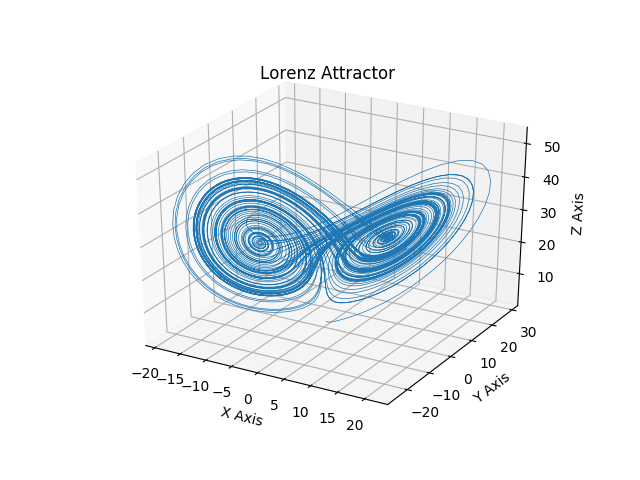
\includegraphics[width=0.6\textwidth]{figures/1_chaotic_lorenz.png}
    \caption{Chaotic solution of the Lorenz attractor.}
\end{figure}
